\RequirePackage{amsmath}
\documentclass{llncs}
\usepackage[utf8]{inputenc}
\PassOptionsToPackage{table}{xcolor}
\pagestyle{headings}  % This option shows page numbers, it have to be removed in the final document.
\usepackage{booktabs}
\usepackage{amssymb}
\usepackage{tikz}
\usepackage{scalerel}
\usepackage{comment}
\usepackage{framed}
\usepackage{listings}
\usepackage{mathtools}
%\usepackage{pifont}% http://ctan.org/pkg/pifont
%\usepackage{balance}
%\usepackage{stmaryrd}
\usepackage{adjustbox}
\usepackage{multirow}
\usepackage{enumitem}
\usepackage{xspace}
\usepackage{url}
\usepackage{inconsolata}
\usepackage{etoolbox}

\renewcommand{\UrlFont}{\ttfamily\scriptsize}

%%%%%%%%%%%%%%%%%%%%%%%%%%%%%%%%%%%%%%%%%%%%%%%%%%%%%%
%% Quickly switch from conference to extended version
\providetoggle{conf}
\settoggle{conf}{false}

% text only to appear in extended version
\newcommand{\ever}[1]{\iftoggle{conf}{}{#1}}

% text only to appear in the conference version
\newcommand{\cver}[1]{\iftoggle{conf}{#1}{}}

% alternate text for both versions
\newcommand{\cever}[2]{\iftoggle{conf}{#1}{#2}}

% environment for long extended-only text
\iftoggle{conf}%
 {\excludecomment{exver}}%
 {\newenvironment{exver}}%
%%%%%%%%%%%%%%%%%%%%%%%%%%%%%%%%%%%%%%%%%%%%%%%%%%%%%% 


\usepackage{floatrow}
% Table float box with bottom caption, box width adjusted to content
\newfloatcommand{capbtabbox}{table}[][\FBwidth]

\newcommand{\ah}[1]{{\color{blue}\textsc{ah:} #1}}

\makeatletter
\renewcommand\paragraph{\@startsection{paragraph}{4}{\z@}%
	{1ex \@plus1ex \@minus.2ex}%
	{-1em}%
	{\normalfont\normalsize\itshape}}

%%%%%%%%%%%%%%%%%%%%%%%%%%%%%%%%%%%%%%%%%%%%%%%%%
% SPARQL Listing style
%%%%%%%%%%%%%%%%%%%%%%%%%%%%%%%%%%%%%%%%%%%%%%%%%
\usepackage{listings}

\colorlet{punct}{red!60!black}
\definecolor{background}{HTML}{EEEEEE}
\definecolor{delim}{RGB}{120,20,40}
\definecolor{keyw}{RGB}{0,0,192}
\colorlet{numb}{magenta!60!black}

\lstdefinelanguage{sparql}{
	sensitive=false,
	extendedchars=true,
	literate={á}{{\'a}}1 {é}{{\'e}}1 {í}{{\'{\i}}}1 {ó}{{\'o}}1 {ú}{{\'u}}1
	{Á}{{\'A}}1 {É}{{\'E}}1 {Í}{{\'I}}1 {Ó}{{\'O}}1 {Ú}{{\'U}}1
	{ü}{{\"u}}1 {Ü}{{\"U}}1 {ñ}{{\~n}}1 {Ñ}{{\~N}}1 {¿}{{?``}}1 {¡}{{!``}}1
	{<}{{{\color{delim}<}}}{1}
	{>}{{{\color{delim}>}}}{1}
	{?}{{{\color{delim}?}}}{1}
	{*}{{{\color{delim}*}}}{1}
	{+}{{{\color{delim}+}}}{1}
	{/}{{{\color{delim}/}}}{1}
	{,}{{{\color{punct}{,}}}}{1}
	{;}{{{\color{punct}{;}}}}{1}
	{.}{{{\color{punct}{.}}}}{1}
	{:}{{{\color{punct}{:}}}}{1}
	{\{}{{{\color{delim}{\{}}}}{1} {\}}{{{\color{delim}{\}}}}}{1},
	morekeywords={ask,select,from,where,order,by,distinct,limit,offset,optional,union,filter,prefix,bound,desc,regex,str,group,not,exists,minus,service,certain,maybe}
}

\lstdefinestyle{sparqld}{
	basicstyle=\scriptsize\ttfamily,
	identifierstyle=\color{black},
	keywordstyle=\color{keyw}\bfseries,
	ndkeywordstyle=\color{greenCode}\bfseries,
	stringstyle=\color{ocherCode}\ttfamily,
	commentstyle=\color{darkgray}\ttfamily,
	language={sparql},
	tabsize=2,
	showtabs=false,
	showspaces=false,
	showstringspaces=false,
	extendedchars=true,
	escapechar=`,
	frame={single},
	breaklines=true,
	basewidth=0.5em,
	moredelim=[is][\color{magenta}]{~}{~},
	moredelim=**[is][\color{gray}]{£}{£},
	moredelim=**[is][\color{blue!50!black}]{$}{$},
	moredelim=[is][\color{orange!80!black}]{!}{!},
	moredelim=**[is][\color{green!50!black}]{¬}{¬},
	xleftmargin=2ex,
	xrightmargin=1ex,
	aboveskip=1.5ex,
	belowskip=1.5ex
}

\makeatletter
\newcommand{\sqbox}{%
	\collectbox{%
		\@tempdima=\dimexpr\width-\totalheight\relax
		\ifdim\@tempdima<\z@
		\fbox{\hbox{\hspace{-.5\@tempdima}\BOXCONTENT\hspace{-.5\@tempdima}}}%
		\else
		\ht\collectedbox=\dimexpr\ht\collectedbox+.5\@tempdima\relax
		\dp\collectedbox=\dimexpr\dp\collectedbox+.5\@tempdima\relax
		\fbox{\BOXCONTENT}%
		\fi
	}%
}
\makeatother
%%%%%%%%%%%%%%%%%%%%%%%%%%%%%%%%%%%%%%%%%%%%%%%%%
% /SPARQL Listing style
%%%%%%%%%%%%%%%%%%%%%%%%%%%%%%%%%%%%%%%%%%%%%%%%%

%%%%%%%%%%%%%%%%%%%%%%%%%%%%%%%%%%%%%%%%%%%%%%%%%
% TiKz for RDF graphs
%%%%%%%%%%%%%%%%%%%%%%%%%%%%%%%%%%%%%%%%%%%%%%%%%

\usetikzlibrary{shapes,arrows,positioning,fit,backgrounds,matrix,chains,scopes,calc}

\newcommand{\hsp}{\vphantom{Ag}}
\tikzset{
	std/.style={ 
		draw,
		circle,
		anchor=center,
		inner sep=0pt,
		minimum size=5pt
	},
	lab/.style={ 
		text centered,
		fill=white, 
		inner sep=0.7pt,
		font=\tt\small\hsp},
	iri/.style={
		draw=black!50!white, 
		rectangle,
		rounded corners,
		thick,
		text centered,
		top color=white, 
		bottom color=black!15,
		%opacity=0.7,
		%text opacity=1,
		font=\tt\small\hsp,
		anchor=center},
	lit/.style={
		draw=black!50!white, 
		rectangle,
		thick,
		text centered,
		top color=white, 
		bottom color=black!15, 
		anchor=center,
		%opacity=0.7,
		%text opacity=1,
		font=\tt\small\hsp},
	arrout/.style={
		->,
		-latex,
		%draw=black!50, 
		%fill=black!50,
		%thick,
		font=\tt\small\hsp},
	arrin/.style={
		<-,
		latex-,
		%draw=black!50, 
		%fill=black!50,
		%thick,
		font=\tt\small\hsp},
	arrinout/.style={
		<->,
		latex-latex,
		%draw=black!50, 
		%fill=black!50,
		%thick,
		font=\tt\small\hsp},
	arrstd/.style={
		-,
		%draw=black!50, 
		%fill=black!50,
		thick},
	dashmed/.style={
		-,
		%draw=black!50, 
		%fill=black!50,
		thick,
		dash pattern=on 3pt off 3pt,
		font=\tt\small\hsp},
	fade/.style={
		opacity=0.4,
		text opacity=0.4
	},
	fadet/.style={
		opacity=1,
		text opacity=0.4
	},
	every loop/.style={
		<-,
		latex-,
		fill=black!50,
		min distance=10mm,
		in=0,
		out=60,
		looseness=10,
		draw=black!50,
		thick,
		font=\tt\small\hsp
	},
	lean/.style={
		dotted,
		blue
	},
	leane/.style={
		dotted,
		blue
	},
	leanl/.style={
		text=blue
	}	
}

\newlength{\hgap}
\newlength{\vgap}
\setlength{\hgap}{2cm}
\setlength{\vgap}{1.2cm}

%%%%%%%%%%%%%%%%%%%%%%%%%%%%%%%%%%%%%%%%%%%%%%%%%
% /TiKz for RDF graphs
%%%%%%%%%%%%%%%%%%%%%%%%%%%%%%%%%%%%%%%%%%%%%%%%%

%%%%%%%%%%%%%%%%%%%%%%%%%%%%%%%%%%%%%%%%%%%%%%%%%
% PGFplots
%%%%%%%%%%%%%%%%%%%%%%%%%%%%%%%%%%%%%%%%%%%%%%%%%
\usepackage{pgfplots}
\usepgfplotslibrary{groupplots}
\usepackage{pgfplotstable}
\pgfplotsset{compat=newest}
\usetikzlibrary{pgfplots.statistics}

\makeatletter
\pgfplotsset{
	boxplot prepared from table/.code={
		\def\tikz@plot@handler{\pgfplotsplothandlerboxplotprepared}%
		\pgfplotsset{
			/pgfplots/boxplot prepared from table/.cd,
			#1,
		}
	},
	/pgfplots/boxplot prepared from table/.cd,
	table/.code={\pgfplotstablecopy{#1}\to\boxplot@datatable},
	row/.initial=0,
	make style readable from table/.style={
		#1/.code={
			\pgfplotstablegetelem{\pgfkeysvalueof{/pgfplots/boxplot prepared from table/row}}{##1}\of\boxplot@datatable
			\pgfplotsset{boxplot/#1/.expand once={\pgfplotsretval}}
		}
	},
	make style readable from table=lower whisker,
	make style readable from table=upper whisker,
	make style readable from table=lower quartile,
	make style readable from table=upper quartile,
	make style readable from table=median,
}
\makeatother

%%%%%%%%%%%%%%%%%%%%%%%%%%%%%%%%%%%%%%%%%%%%%%%%%
% /PGFplots
%%%%%%%%%%%%%%%%%%%%%%%%%%%%%%%%%%%%%%%%%%%%%%%%%

\usepackage{arydshln}

%%%%%%%%%%%%%%%%%%%%%%%%%%%%%%%%%%%%%%%%%%%%%%%%%
% Hyperref
%%%%%%%%%%%%%%%%%%%%%%%%%%%%%%%%%%%%%%%%%%%%%%%%%
\usepackage{hyperref}
\definecolor{dark-blue}{rgb}{0.0,0.0,0.2}
\definecolor{dark-green}{rgb}{0.0,0.2,0.0}
\definecolor{dark-red}{rgb}{0.2,0.0,0.0}
\hypersetup{
	colorlinks, linkcolor={dark-red},
	citecolor={dark-green}, urlcolor={dark-blue},
	pdftitle={Versioned Queries over RDF Archives: All You Need is SPARQL?},    % title
	pdfauthor={Ignacio Cuevas, Aidan Hogan},     % author
	pdfsubject={MEPDaW 2020: Managing the Evolution and Preservation of the Data Web},   % subject of the document
	pdfkeywords={sparql;} {versioning;} {rdf archives;} {dynamics}, % list of keywords
}

%%%%%%%%%%%%%%%%%%%%%%%%%%%%%%%%%%%%%%%%%%%%%%%%%
% /Hyperref
%%%%%%%%%%%%%%%%%%%%%%%%%%%%%%%%%%%%%%%%%%%%%%%%%


%%%%%%%% MACROS

\newcommand{\B}{\ensuremath{\mathbf{B}}\xspace}
\newcommand{\I}{\ensuremath{\mathbf{I}}\xspace}
\renewcommand{\L}{\ensuremath{\mathbf{L}}\xspace}
\newcommand{\V}{\ensuremath{\mathbf{V}}\xspace}

\newcommand{\cpx}[2]{\ensuremath{\textsc{#1-}\mathrm{#2}}\xspace}
\newcommand{\npc}{\cpx{NP}{complete}}
\newcommand{\nph}{\cpx{NP}{hard}}
\newcommand{\psc}{\cpx{PSpace}{complete}}
\newcommand{\psh}{\cpx{PSpace}{hard}}
\newcommand{\gic}{\cpx{GI}{complete}}
\newcommand{\gih}{\cpx{GI}{hard}}
\newcommand{\dpc}{\cpx{DP}{complete}}
\newcommand{\dph}{\cpx{DP}{hard}}
\newcommand{\conpc}{\cpx{coNP}{complete}}
\newcommand{\conph}{\cpx{coNP}{hard}}
\newcommand{\ptp}{\ensuremath{\Pi_2^P}}
\newcommand{\ptph}{\cpx{\ptp}{hard}}
\newcommand{\ptpc}{\cpx{\ptp}{complete}}

\newcommand{\tch}[1]{\textbf{#1}}
\newcommand{\rid}[1]{\textsc{#1}}
\newcommand{\ttl}[1]{\textsf{#1}}
\newcommand{\tid}[1]{\textsc{#1}}
%\newcommand{\dom}{\tid{dom}}
%\newcommand{\rng}{\tid{rng}}
%\newcommand{\sC}{\tid{sC}}
%\newcommand{\sP}{\tid{sP}}

\newcommand{\ssyn}[3]{[\ensuremath{#1\,\textsc{#2}\,#3}]}
\newcommand{\sand}[2]{\ssyn{#1}{and}{#2}}
\newcommand{\suni}[2]{\ssyn{#1}{union}{#2}}
\newcommand{\sopt}[2]{\ssyn{#1}{opt}{#2}}
\newcommand{\sminus}[2]{\ssyn{#1}{minus}{#2}}
\newcommand{\sfil}[2]{\ensuremath{\textsc{filter}_{#2}(#1)}}
\newcommand{\ssel}[2]{\ensuremath{\textsc{select}_{#2}#1}}
\newcommand{\sseld}[2]{\ensuremath{\textsc{select}^\Delta_{#2}#1}}
\newcommand{\sfrom}[3]{\ensuremath{\textsc{from}_{#2,#3}#1}}
\newcommand{\dom}[1]{\ensuremath{\mathrm{dom}(#1)}}
\newcommand{\vars}[1]{\ensuremath{\mathrm{vars}(#1)}}
\newcommand{\can}[1]{\ensuremath{\mathrm{can}(#1)}}
\newcommand{\com}[2]{\ensuremath{#1 \sim #2}}

%\newcommand{\hsc}[1]{{\footnotesize\MakeUppercase{#1}}}
\newcommand{\hsc}[1]{#1}

%\newcommand{\utp}[1]{\textsc{tp}{(#1)}}
\newcommand{\ufo}[1]{\textsf{\hsc{\upshape #1}}}
\newcommand{\uand}[1]{\ensuremath{\ufo{and}(#1)}}
\newcommand{\uuni}[1]{\ensuremath{\ufo{union}(#1)}}
\newcommand{\usel}[2]{\ensuremath{\ufo{select}_{#2}(#1)}}
\newcommand{\useld}[2]{\ensuremath{\ufo{select}^\Delta_{#2}(#1)}}

\newcommand{\uandn}{\ensuremath{\ufo{and}}}
\newcommand{\uunin}{\ensuremath{\ufo{union}}}

\newcommand{\bn}[1]{\texttt{\_:#1}}
\newcommand{\iri}[1]{\texttt{:#1}}
\newcommand{\var}[1]{\texttt{?#1}}

\newcommand{\ican}[1]{\ensuremath{\textsc{iCan}(#1)}}
\newcommand{\ecan}[1]{\ensuremath{\textsc{eCan}(#1)}}

\newcommand{\ev}[2]{\ensuremath{#1(#2)}}

\def\ojoin{\setbox0=\hbox{$\bowtie$}%
	\rule[0.18ex]{.25em}{.5pt}\llap{\rule[.9ex]{.25em}{.5pt}}}
\def\loj{\mathbin{\ojoin\mkern-5.8mu\bowtie}}

\newcommand{\da}{\ensuremath{:\nolinebreak\mkern-1.2mu\nolinebreak=}}

\newcommand{\qedr}{\begin{flushright}\qed\end{flushright}}

\newcommand{\yt}{\ding{51}}%
\newcommand{\nt}{\ding{55}}%

\newcommand{\para}[1]{\smallskip\noindent\textbf{#1:}}

\newcommand{\mq}{\textsc{mq}\xspace}
\newcommand{\mqs}{\textsc{mq}s\xspace}
\newcommand{\ucq}{\textsc{ucq}\xspace}
\newcommand{\ucqs}{\textsc{ucq}s\xspace}
\newcommand{\cq}{\textsc{cq}\xspace}
\newcommand{\cqs}{\textsc{cq}s\xspace}
\newcommand{\cuq}{\textsc{ucq}\xspace}
\newcommand{\cuqs}{\textsc{ucq}s\xspace}

%%%%%%%%

\graphicspath{ {images/} }	

\begin{document}
\title{Versioned Queries over RDF Archives:\\All You Need is SPARQL?}

\author{Ignacio Cuevas \and Aidan Hogan}
\institute{Department of Computer Science, University of Chile \& IMFD Chile}

\maketitle

\begin{abstract}
Although many prominent Linked Datasets are in a state of constant evolution, historical data are rarely published in a standard way. Though a number of works have recently addressed the issue of querying and managing archives of versioned RDF data, most propose dedicated solutions, which incurs a high deployment cost. We rather explore solutions for representing archives of versioned RDF data using the SPARQL standard without modification, allowing existing implementations to be used. For querying, we consider two versioning primitives: viewing results from a particular version, or viewing results that change between two consecutive versions. We identify and compare several models by which historical versions of an RDF graph can be stored as named graphs, and discuss how base queries can be rewritten in each model per the two aforementioned primitives. We then present a performance comparison of these models and baseline (non-)versioned queries with respect to 23 weekly versions of Wikidata and 232 user-defined queries, using Virtuoso as a reference SPARQL implementation.
\end{abstract}


\section{Introduction}

A key aspect of the Web is its dynamic nature, where documents are frequently updated, deleted and added. Likewise when we speak of the Semantic Web, it is important to consider that sources may be dynamic and RDF datasets are subject to change~\cite{KaferAUOH13}. It is in this context that various works have looked at versioning in the context of RDF/SPARQL~\cite{VolkelG06,TappoletB09,Grandi10,GraubeHU14,KhuranaD16}, with recent works proposing \textit{RDF archives}~\cite{FernandezPU15,Cerdeira-PenaFF16,BahriLA18,FernandezUPK19,TaelmanSHMV19} that manage RDF graphs and their historical changes, allowing for querying across different versions of the graph. Within these works, a variety of specialised indexing techniques~\cite{Cerdeira-PenaFF16,BahriLA18,TaelmanSHMV19}, query languages~\cite{TappoletB09} and benchmarks~\cite{KotsevMPEFK16,FernandezUPK19} have been proposed, developed and evaluated. While these represent important advances, many such proposals are by their nature incompatible with the existing SPARQL infrastructure. Furthermore, benchmarks have mostly focused on synthetic data. Hence there is still a considerable gap between these research works and putting RDF archives into practice.

%The traditional Web and the Semantic Web thus share similar strengths and limitations regarding the dynamics of information. In terms of strengths, the flexible nature of both webs means that documents can be updated with little restriction and with little need for centralised coordination. On the other hand, in terms of limitations, neither web has built in support for preservation, nor for versioning; for example, on the traditional Web, the HTTP protocol does not permit requesting a past version of a webpage. For this reason, a number of specialised ``Web archives'' have emerged that attempt to capture and track different intermittent versions of documents on the Web, the most prominent of which is the Internet Archive~\cite{JaffeK09}. While similar techniques can be applied to Semantic Web documents containing RDF data -- simply archiving and thus preserving the syntax of the document itself -- the structured nature of such content means that an RDF archive can potentially do a lot more.

%A number of works have looked at tracking the dynamics of RDF data on the Web. One such example is the Dynamic Linked Data Observatory (DyLDO)~\cite{KaferAUOH13}, which has been tracking and archiving weekly changes in a diverse sample of RDF documents since 2013. 

In order to bridge this gap, we highlight that -- in theory at least -- there is no need for specialised indexes, query languages, etc., but rather that the types of versioned queries proposed in the literature~\cite{FernandezPU15} can be supported using off-the-shelf SPARQL engines that already enjoy years of development, optimisation, etc., as well as broad deployment on the Web. For example, SPARQL named graphs can be used to track different versions of individual graphs. However, as Fernandez at al.~\cite{FernandezUPK19} note, the approach of using pure SPARQL would ``\textit{typically render rather inefficient SPARQL queries}''. This claim raises the research question: how inefficient will pure SPARQL be in this setting? Though Fernandez at al.~\cite{FernandezUPK19} do discuss how pure SPARQL could be used, to the best of our knowledge, this question has not been empirically explored. If a pure SPARQL solution could be found with relatively little overhead versus base queries (over a single current version) then the benefits would be significant in terms of being able to leverage existing SPARQL infrastructure -- i.e., languages, protocols, implementations -- for managing and querying RDF archives.

In this paper, we present preliminary empirical results addressing this research question. Specifically we take the Virtuoso SPARQL engine~\cite{Erling12} and  evaluate five different representations of RDF archives for XX different weekly versions of truthy Wikidata dumps~\cite{VrandecicK14}. We then implement query rewriting mechanisms for each representation in order to support single-version queries and sequential single-delta queries that retrieve all solutions over an indicated version and all solutions that differ between two sequential versions, respectively. We then perform experiments to compare the sizes of indexes, the costs of indexing new versions, and the costs of query evaluation for base queries over the current version versus rewritten versioned queries.

%Other works rather focus on aspects relating to detecting change~\cite{TummarelloMBE07,ZeginisTC11,PapavasileiouFFKC13,KaferAUOH13,DividinoKG14,RoussakisCSFS15,NishiokaS18}, notifying changes~\cite{TummarelloMBE07,PopitschH11,PassantM10,TrampFEA10}, versioning data~\cite{VolkelG06,GraubeHU14,KhuranaD16}, and so forth. A more recent development is that of RDF archives~\cite{FernandezPU15,Cerdeira-PenaFF16,FernandezUPK19}



%Currently, a large number of existing datasets are based on RDF due to its extense popularity, Wikidata being one the most notorious. Wikidata~\cite{VrandecicK14} is a massive dataset, with over 42 million items~\footnote{\url{https://www.wikidata.org/wiki/Wikidata:Statistics}}, which is based on all the available data of Wikipedia and structured on RDF.
%
%
%Wikidata is in constant change, due to it being an open dataset that allows being edited by users. Furthermore, data is being added often, which makes Wikidata very dynamic in some areas. Given those circumstances, it can be said that Wikidata has many ``versions'' over time, where different data is available at different time intervals, making it possible to analyze its time component.
%
%
%Dataset versioning in RDF/SPARQL is a research topic yet to be fully explored. While there are a number of implementations, most of them rely on specialized indices or SPARQL extensions. As such, it would be relevant to study the possibility of developing a versioning system and methodology for queries using only base SPARQL.
%
%
%Such system could be used as version control for the dataset; administrators would be able to detect erroneous or malicious editions on data that doesn't normally change. On top of that, it would be possible to analyze the evolution of data, possibly predicting future changes. The system could also be used on datasets other than Wikidata, where data history may be poorly (or not at all) preserved.

\section{Related Work}

Various temporal extensions for RDF/SPARQL have been proposed in literature. Gutierrez et al.~\cite{GutierrezHV07} describe a framework that allows time representation in RDF using annotations. Pugliese et al.~\cite{PuglieseUS08} more generally explore time annotations in RDF, proposing semantics, queries and specialised indexes. Zimmerman et al.~\cite{ZimmermannLPS12} provide a general framework for annotating RDF that generalises temporal annotations; they further propose a query language called AnQL for querying annotated RDF. Proposed temporal extensions for SPARQL include $\tau$-SPARQL~\cite{TappoletB09}, T-SPARQL~\cite{Grandi10}, SPARQL-ST~\cite{PerryJS11}, SPARQL\textsuperscript{T}~\cite{ZanioloGACG18}, etc. Related to temporality, a number of systems support versioning for RDF, including SemVersion~\cite{VolkelG06}, POI~\cite{TzitzikasTA08}, x-RDF-3x~\cite{NeumannW10}, R43ples~\cite{GraubeHU14}, Dydra~\cite{AndersonB16} and Ostrich~\cite{TaelmanSV18}. 

More recently the concept of RDF archives have been gaining more and more attention. Fernandez et al.~\cite{FernandezPU15} provide a general survey and introduction to the theme, discussing the types of queries that one might wish to answer in the context of an RDF archive. Works by Cerdeira{-}Pena et al.~\cite{Cerdeira-PenaFF16}, Zaniolo et al.~\cite{ZanioloGACG18} and Taelman et al.~\cite{TaelmanSHMV19} propose ways to compress and index RDF archives, while Khurana and Deshpande~\cite{KhuranaD16} propose indexes more generally for historical graph data. Bahri et al.~\cite{BahriLA18} explore the benefits of using Apache Spark to manage RDF archives in a distributed setting. In order to evaluate these emerging techniques, a number of benchmarks have been proposed, including the BEnchmark of RDF
ARchives (BEAR)~\cite{FernandezUPK19}, and the Semantic Publishing Benchmark (SPB)~\cite{Papakonstantinou18}.

In summary, the past years have seen a wide range of developments in terms of representations, languages, vocabularies, indexes, algorithms, etc., for managing and querying over temporal and/or versioned RDF data. However, to the best of our knowledge, most of these approaches propose specialised languages, implementations, etc., for these purposes. Such languages have the benefit of allowing to more concisely and intuitively express versioned queries, while such implementations can develop optimised techniques that leverage particular characteristics of versioned data. The downside of these specialised approaches is that they are often diverge from practice, requiring the use of research prototypes rather than established SPARQL implementations, non-standard languages, etc. A number of authors have acknowledged that one can manage and query RDF archives using vanilla SPARQL, though it may lead to prolix or inefficient queries~\cite{TappoletB09,FernandezUPK19}; however, we are not aware of any empirical results along these lines. Our work presents some preliminary results that aim to fill this gap and to better understand the costs and limitations of using vanilla SPARQL to host RDF archives.


%An important distinction to make is that their work is focused on \textbf{labeling} over \textbf{versioning}; \textbf{labeling} means adding meta-data to query result validity, meanwhile \textbf{versioning} implies simultaneously keeping several versions of the same dataset. This work also formally defines labels and time intervals, but does not cover an implementation for either.


%Zimmerman et al.~\cite{DBLP:journals/ws/ZimmermannLPS12} extend RDF, allowing the use of generalized annotations, which can be used to represent time intervals and associated to each triple to represent their validity. Same as the previously mentioned work, the objectives seeked by Zimmerman et al. do not completely align with the present work, due to the fact that an RDF extension is used. It will, however, be considered to compare results.


%Grandi~\cite{Grandi10} proposes an extension for SPARQL, including a time component in queries. No implementation details are provided, however. The methodology used for building timed queries will be compared to the one this work defines.


%The prior three works share their focus on formal definitions over implementations. They also do not consider efficiency or scalability analysis and employ SPARQL extensions and/or specialized indices. In light of these facts, said works will be considered only to compare results for the most part.


%Lastly, Tappolet and Bernstein~\cite{TappoletB09} add a time component to RDF's syntax, proposing an eficient method to make SPARQL queries on it, as well. The dataset is annotated with time intervals corresponding to each triple's validity, and a specialized index compliments the query engine. Since this is an alternative solution to the explored challenge, it will be used to compare results, while also evaluating whether their specialized index is necessary and if similar results can be achieved using standar SPARQL.

% \cite{ArndtNRMM19} GIT for RDF

% \cite{Papakonstantinou18} Benchmark results

% \cite{PelgrinGH20}

\section{Preliminaries}

We first establish some preliminaries and notation. RDF triples are composed of three sets of terms: IRIs (\I), literals (\L) and blank nodes (\B). In this preliminary work, we do not consider blank nodes, whose special semantics complicates the detection of changes in RDF graphs~\cite{ZeginisTC11}. Leaving aside blank nodes, an RDF triple $(s,p,o) \in \I \times \I \times (\I \cup \L)$ consists of a subject $s$, predicate $p$ and object $o$. An RDF graph $G$ is then a set of triples. An RDF archive is a tuple of RDF graphs $\mathcal{G} = (G_1,\ldots,G_n)$, interpreted as $n$ sequential versions of a given RDF graph. 

A triple pattern $(s,p,o) \in (\I \cup \V) \times (\I \cup \V) \times (\I \cup \L \cup \V)$ is an RDF triple that permits variables from a set $\V$ to appear in any position. A solution is a partial mapping $\mu : \V \rightarrow \I \cup \L$. We denote by $\dom{\mu}$ the \textit{domain} of $\mu$, i.e., the set of variables for which $\mu$ is defined. We say that two solutions $\mu_1, \mu_2$ are compatible, denoted $\mu_1 \sim \mu_2$, if and only if $\mu_1(v) = \mu_2(v)$ for all $v \in \dom{\mu_1} \cap \dom{\mu_2}$.

A basic graph pattern $B$ is a set of triple patterns. Let $\vars{B}$ denote the set of variables appearing in $B$ and let $\mu(B)$ denote the image of $B$ under $\mu$, i.e., the result of replacing all variables $v \in \dom{\mu} \cap \vars{B}$ with $\mu(v)$ in $B$. The evaluation of a basic graph pattern $B$ on an RDF graph $G$ is given as $B(G) \coloneqq \{ \mu \mid \mu(B) \subseteq G\text{ and }\dom{\mu} = \vars{B} \}$.

SPARQL queries are based on basic graph patterns and a number of relational operators. Similar to Pérez et al.~\cite{PerezAG09}, we define an abstract syntax for a subset of SPARQL of pertinence to this paper as follows. A basic graph pattern $B$ is a graph pattern. Furthermore, if $P$ and $Q$ are graph patterns, and $V \subset \V$ is a set of variables, then $\sand{P}{Q}$, $\suni{P}{Q}$, $\sminus{P}{Q}$ and $\ssel{P}{V}$ are graph patterns. We define the semantics of these graph patterns in Table~\ref{tab:sparql}.

\begin{table}[t]
{\scriptsize
\begin{align*}
\sand{P}{Q}(G) \da &\, P(G) \Join Q(G) & M_1 \Join M_2 \da &\, \{ \mu_1 \cup \mu_2 \mid \mu_1 \in M_1,\, \mu_2 \in M_2,\, \com{\mu_1}{\mu_2} \} \\
\suni{P}{Q}(G) \da &\, P(G) \cup Q(G) & M_1 \cup M_2 \da &\, \{ \mu \mid \mu \in M_1\text{ or }\mu \in M_2 \} \\
\sminus{P}{Q}(G) \da &\, P(G) \setminus Q(G) &  M_1 \setminus M_2 \da &\, \{ \mu_1 \in M_1 \mid \nexists \mu_2 \in M_2 : \com{\mu_1}{\mu_2} \} \\
%M_1 \loj M_2 \da\, & (M_1 \bowtie M_2) \cup (M_1 \setminus M_2) \\
%\sigma_R(M) \da\,& \{ \mu \in M \mid \mu \models R \}\\
\ssel{P}{V}(G) \da &\, \pi_V(P(G)) & \pi_V(M) \da\,& \{ \mu' \mid \exists \mu \in M : \mu' \sim \mu, \dom{\mu'} = V \cap \dom{\mu} \}
\end{align*}}
\caption{Semantics for SPARQL query operators where $M$, $M_1$ and $M_2$ denote sets of solutions, $V$ denotes a set of variables\label{tab:sparql}}
\end{table}

In this paper, we rely not only on RDF graphs, but also on SPARQL datasets to represent RDF archives. A SPARQL dataset $D \coloneqq \{ G, (n_1,G_1), \ldots (n_m,G_m) \}$ consists of a default (RDF) graph $G$ and a set of named graphs, each being a pair $(n_i,G_i)$ where $n_i \in \I$, $G_i$ is an RDF graph, and $n_i \neq n_j$ for $1 \leq i \leq m$, $1 \leq j \leq m$, $i \neq j$. For simplicity, we will consider a SPARQL dataset $D$ to be a set of quads of the form $(G \times \{*\}) \cup (G_1 \times \{n_1\}) \cup \ldots \cup (G_m \times \{n_m\})$, where $* \notin \I \cup \L \cup \V$ is a special symbol denoting the default graph.\footnote{We thus assume a \textit{quad store}, and disallow empty named graphs.} Different named graphs can be queried using a \texttt{GRAPH} operator, creating quad patterns. A quad pattern $(s,p,o,g) \in (\I \cup \V) \times (\I \cup \V) \times (\I \cup \L \cup \V) \times (\I \cup \{ *\})$ extends a triple pattern with a fourth element that may be an IRI or *. A basic named graph pattern $C$ is then a set of quad patterns whose evaluation on an SPARQL dataset $D$ is given as $C(D) \coloneqq \{ \mu \mid \mu(C) \subseteq D\text{ and }\dom{\mu} = \vars{C} \}$. Following the SPARQL standard~\cite{sparql11}, we translate a triple pattern $(s,p,o)$ to a quad pattern $(s,p,o,*)$ such that it is evaluated only on the default graph.\footnote{In concrete SPARQL syntax, quad patterns are expressed with the $\texttt{GRAPH}$ keyword.} The semantics of the operators defined in Table~\ref{tab:sparql} then remain unchanged simply allowing $P$ and $Q$ to now represent basic named graph patterns, defined to be graph patterns.

SPARQL provides two operators to initialise a SPARQL dataset: \texttt{FROM} and \texttt{FROM NAMED}. We combine both for brevity into one operator. A graph pattern $P$ is considered to be a query. Likewise if $P$ is a graph pattern, and $M$ and $N$ are sets of IRIs, then $\sfrom{P}{M}{N}$ is also a query. The evaluation of $\sfrom{P}{M}{N}$ on a dataset $D$ is defined as $\sfrom{P}{M}{N}(D) \coloneqq P(D_{M,N})$, where the query dataset $D_{M,N} \coloneqq (\cup_{m \in M} D(m) \times \{ *\}) \cup  (\cup_{n \in N} D(n) \times n)$ is formed from a default graph containing the union\footnote{Since we do not allow blank nodes, a union or RDF merge is equivalent.} of graphs with a name $m \in M$, and all the named graphs in $D$ with a graph named $n \in N$. We will be able to use these operators to define query datasets that capture specific versions in an RDF archive.

\section{Versioned Data}

Our general approach is to represent an RDF archive as a SPARQL dataset $D$ but there are multiple representations by which this can be achieved, each with its own strength and weaknesses. We propose six different representations falling into three different categories as discussed by various authors (e.g.,~\cite{TzitzikasTA08,FernandezPU15}): \textit{Independent Copies} (\textit{IC}), \textit{Change-Based} (\textit{CB}) and \textit{Timestamp-Based} (\textit{TB}).

\newcommand{\ic}{\textsc{i}\xspace}
\newcommand{\cbpd}{\ensuremath{\textsc{c}_d^{+}}\xspace}
\newcommand{\cbpi}{\ensuremath{\textsc{c}_i^{+}}\xspace}
\newcommand{\cbmd}{\ensuremath{\textsc{c}_d^{-}}\xspace}
\newcommand{\cbmi}{\ensuremath{\textsc{c}_i^{-}}\xspace}
\newcommand{\cbi}{\ensuremath{\textsc{c}_i}\xspace}
\newcommand{\cbd}{\ensuremath{\textsc{c}_d}\xspace}
\newcommand{\cbp}{\ensuremath{\textsc{c}^{+}}\xspace}
\newcommand{\cbm}{\ensuremath{\textsc{c}^{-}}\xspace}
\newcommand{\tb}{\textsc{t}\xspace}

\paragraph{Independent Copies (IC):} Perhaps the most intuitive representation is to store each constituent graph of an RDF Archive $\mathcal{G} = (G_1,\ldots,G_n)$ as a SPARQL dataset $D = \{ (x_1,G_1), \ldots, (x_n,G_n)\}$, where $x_1,\ldots,x_n$ are IRIs that deterministically identify the version. This will result in relatively simple (and thus likely efficient) rewritten queries, but can be expected to occupy a lot of space, particularly in cases where a small proportion of triples change from version to version. We thus consider the $IC$ representation to be a baseline for comparison.

\paragraph{Change-Based (CB):} The core idea of $CB$ representations is to store only triples that change from a given reference version. Along these lines, in the following we denote by $\Delta_{i}^j \coloneqq G_i \setminus G_j$ the triples in version $i$ not in version $j$. We then consider four $CB$ representations based on the following transformations of an RDF archive $\mathcal{G} = (G_1,\ldots,G_n)$:
%
{\footnotesize
\begin{align*}
\mathcal{G}^n_1 \da\,& (G_1,\Delta_1^2,\Delta_2^1,\ldots,\Delta_1^n,\Delta_n^1) & G_i & = (G_1 \cup \Delta_i^1) \setminus \Delta_1^i & \text{for }1 < i \leq n\\
\mathcal{G}^n_{n-1} \da\,& (G_1,\Delta_1^2,\Delta_2^1,\ldots,\Delta_{n-1}^n,\Delta_n^{n-1}) & G_i & = (G_{i-1} \cup \Delta_i^{i-1}) \setminus \Delta_{i-1}^i & \text{for }1 < i \leq n \\
\mathcal{G}^1_n \da\,& (G_n,\Delta_n^{n-1},\Delta_{n-1}^n,\ldots,\Delta_n^1,\Delta_1^n) & G_i & = (G_n \cup \Delta_i^n) \setminus \Delta_n^i & \text{for }1 \leq i < n \\
\mathcal{G}^{n-1}_n \da\,& (G_n,\Delta_n^{n-1},\Delta_{n-1}^n,\ldots,\Delta_2^1,\Delta_1^2) & G_i & = (G_{i+1} \cup \Delta_i^{i+1}) \setminus \Delta_{i+1}^i & \text{for }1 \leq i < n
\end{align*}%
}%
%
As can be seen for the definitions of $G_i$, these transformations are lossless: we can retrieve any version of the graph from any such transformation. The first two transformations start with the earliest version as a base. The first encodes deltas always with respect to the first version. The second encodes deltas with respect to the previous version. The latter two transformations start with the latest version. The third encodes deltas with respect to the latest version. The forth encodes deltas with respect to the subsequent version. Letting $\mathcal{H} = (H_1,\ldots,H_n)$ such that $H_i = G_{n-i+1}$ ($1 \leq i \leq n$), i.e., such that $\mathcal{H}$ ``reverses''$\mathcal{G}$, we remark that $\mathcal{G}^n_1 = \mathcal{H}^1_n$ and $\mathcal{G}^n_{n-1} = \mathcal{H}^{n-1}_n$. Each such transformation can then be represented as a SPARQL dataset with $2(n-1)+1$ named graphs.

In terms of space we expect $\mathcal{G}^n_{n-1}$ and $\mathcal{G}^{n-1}_n$ to be the most efficient as they always encode deltas from a neighbouring version. However, in terms of query rewriting, we expect $\mathcal{G}^n_{1}$ and $\mathcal{G}^{1}_n$ to be more efficient as they do not require a recursive construction of all intermediate versions towards the base version. In terms of indexing a new version, we expect $\mathcal{G}^{n}_1$ followed by $\mathcal{G}^{n}_{n-1}$ to be most efficient as they require only computing the most recent deltas; we expect $\mathcal{G}^{1}_n$, followed by $\mathcal{G}^{n-1}_{n}$, to be much more expensive, requiring a recompute of all deltas. On the other hand, $\mathcal{G}^{1}_n$ and $\mathcal{G}^{n-1}_{n}$ should be advantageous for queries over more recent versions, which we could reasonably expect to be the most frequent.\footnote{One may note that these four representations are analogous to differential backups, incremental backups, reverse-differential backups, and reverse-incremental backups.}

\paragraph{Timestamp-Based (TB):} The intuition of the $TB$ representation is to associate each triple with the versions in which it is contained. Along these lines, we denote by $\mathcal{G}(s,p,o) \coloneqq \{ i \mid (s,p,o) \in G_i\text{ for } 1 \leq i \leq n \}$ the versions containing $(s,p,o)$.\footnote{The definition $\mathcal{G} : \I \times \I \times (\I \cup \L) \rightarrow 2^{\{1,\ldots,n\}}$~\cite{FernandezUPK19} is analogous to $\mathcal{G} = (G_1,\ldots,G_n)$.} Let $\mathcal{N} \coloneqq \{ N \mid \exists (s,p,o) \in G_i : \mathcal{G}(s,p,o) = N, 1 \leq i \leq n  \}$ denote the family of sets of versions associated with some triple in $(s,p,o)$. We can then represent the RDF archive with a named graph for each $N \in \mathcal{N}$. However, care must be taken as the number of named graphs could potentially reach $2^n$. Though this worst-case is unlikely to happen in practice (it would require triples often being intermittently added and removed across versions), a more practical option is to apply interval encoding and create a named graph for each interval~\cite{FernandezPU15}. More specifically, a triple $(s,p,o)$ is added to an interval $[i,j]$ (for $1 \leq i \leq j \leq n$) if and only if $(s,p,o) \in G_k$ for $i \leq k \leq j$ and either $i = 1$ or $(s,p,o) \notin G_{i-1}$ and $j = n$ or $(s,p,o) \notin G_{j+1}$; in simpler terms, $[i,j]$ is a maximal contiguous interval of versions in which $(s,p,o)$ appears. The upper bound is now $n(n+1)/2$ named graphs, but with the possibility of ``intermittent'' triples appearing in multiple named graphs for different intervals. Empty intervals can be omitted.

In general, we expect the space to be similar to $\mathcal{G}^n_{n-1}$ and $\mathcal{G}^{n-1}_n$; in other words, quite good. In terms of query rewriting, we would expect performance to be quite good for a low number of versions and few intermittent triples as -- unlike for $CB$ representations -- negation is not required; we can rather take the union of interval graphs containing the version. However, as the number of versions $n$ grows, $O(n^2)$ interval graphs need to be unioned in the worst-case to materialise a particular version; by way of comparison, $CB$ representations require processing $O(1)$ (in the case of $\mathcal{G}^n_1$ and $\mathcal{G}^1_n$) or $O(n)$ (in the case of $\mathcal{G}^n_{n-1}$ and $\mathcal{G}^{n-1}_n$) named graphs to materialise a particular version. 

%There are a fours ways in which this can be done. The first option is to transform the RDF archive $\mathcal{G} = (G_1,\ldots,G_n)$ into a set of deltas relative to the initial version: $\mathcal{G}^1_n = (G_1,\Delta_1^2,\Delta_2^1,\ldots,\Delta_1^n,\Delta_n^1)$, resulting in $2(n-1)+1$ graphs. A particular version $G_i$ can then be reconstructed by applying $(G_1 \cup \Delta_i^1) \setminus \Delta_1^i$.


\section{Versioned Queries}

\begin{verbatim}
?s :p ?o
\end{verbatim}

\section{Experiments} 

We now perform experiments to address the following research questions (Q1) Which of the six representations allow for better compression, more efficient indexing, and more efficient updates of a new version? (Q2) How do the query runtimes of compressed representations (\textit{CB}, \textit{TB}) compare with indexing complete versions (\textit{IC})? (Q3) Which representation works best overall? 

\paragraph{Setting} We address these research questions in the context of a Wikidata archive of 8 weekly truthy versions from 2017-08-09 with 1.506 billion triples, to 2017-09-27 with 1.924 billion triples. The RDF archive thus consists of 13.477 billion versioned triples. Each week 25--93 million triples are added, while 4--6 million triples are removed (an update counts as both an addition and a removal). We base our experiments on the example list of queries contributed by users and members of the Wikidata community, which features a wide variety of query operators, diverse terms, etc.\footnote{\url{https://www.wikidata.org/wiki/Wikidata:SPARQL_query_service/queries/examples}} We translate some of the Wikidata-specific features (e.g., the label service) to standard SPARQL. We further filter queries that feature federation to other endpoints, property paths, and qualifiers (not present in the truthy versions). The result is a test set of 146 SPARQL queries. We choose Virtuoso as our SPARQL implementation since it is widely used and has demonstrated good performance in prior benchmarks over Wikidata~\cite{HernandezHK15}. The runtimes presented are averaged over three runs. A timeout of 5 minutes was set per query.

\paragraph{Indexing} We first look at the results of total index sizes for each representation. In Figure~\ref{fig:index} we show the index sizes (GB) for each representation, the time taken (min.) to bulk load all versions in the representation, and the time taken (min.) to update the archive indexing seven versions with the eighth version. We see that (as expected) \ic has the largest index sizes, followed by \cbpd and \cbmd. followed by \tb, followed by \cbpi and \cbmi with the smallest indexes. We see that for a bulk load, index times correlate with index size, with \ic being by far the slowest due to the greater volume of data to index. Finally, with respect to the version update, we again see a similar trend, except that (as expected) \cbmi is far slower than the other alternatives (even \ic) as the entire archive must be built from scratch relative to the most recent version, taking time comparable to a full bulk load.

\paragraph{Single version queries} We apply the rewriting of our 146 SPARQL queries for each of our six representations in order to retrieve results for version 1, 5 and 8. We show the results as box-plots with log $y$-axis in Figure~\ref{fig:svq}. In general we note that median times were generally in the range of 100-1000~ms, though 1--20 queries timed-out in each experiment, affecting the mean (shown as a diamond). In terms of mean and median runtimes, \ic performs the best, with \cbpd, \cbmd and \tb also performing competitively across the different versions. Conversely, \cbpi and \cbmi perform quite poorly relative to the other options (except \cbmi in the case of version 8, which performs well in the median case). Contrasting the query times with index sizes, we note a clear time--space trade-off, where the largest index performs best, the smallest perform worst, and those with intermediate space perform in the middle of the pack. 

\paragraph{Delta version queries} Next we rewrite our 146 SPARQL queries in order to retrieve delta results between versions 1--2, 4--5 and 7--8 from each of our six representations. We again show the results as box-plots with log $y$-axis in Figure~\ref{fig:dvq}. When compared with single version queries, we see a considerable leap in time, where the median runtimes of even the best performing representations approach or exceed 1000 ms more frequently. This time we note that the best performance is offered by \tb, followed by \ic, \cbpi and \cbmi. Conversely,  \cbpd and \cbmd perform very poorly. In these experiments the incremental builds perform better than differential builds as the incremental deltas directly provide the difference between subsequent versions, providing an additional avenue for optimisation.  


\begin{figure}[t]
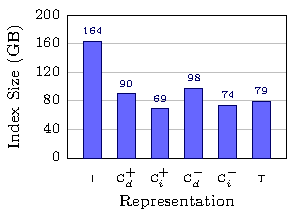
\includegraphics[scale=0.8]{plots/indexsize}
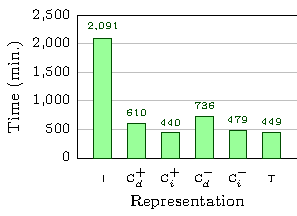
\includegraphics[scale=0.8]{plots/indextime}
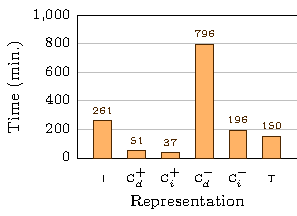
\includegraphics[scale=0.8]{plots/updatetime}
\caption{Indexing details including size (left), bulk load (mid) and version update (right) \label{fig:index}}
\end{figure}

\begin{figure}[t]
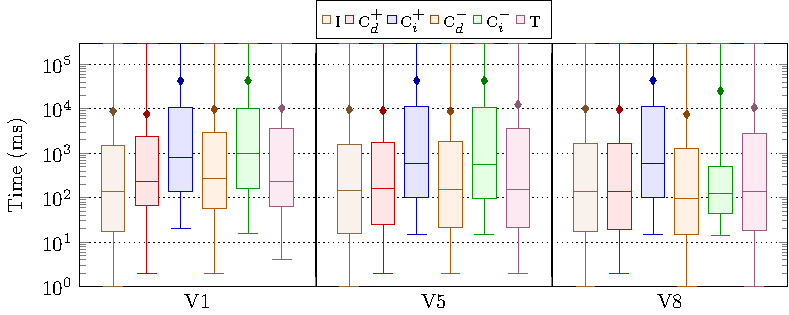
\includegraphics[scale=0.8]{plots/boxplt-svq}
\caption{Single version query times for version 1 (left), 5 (mid) and 8 (right) \label{fig:svq}}
\end{figure}

\begin{figure}[t]
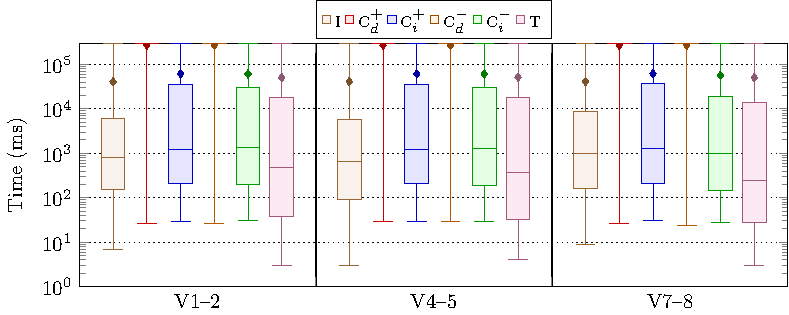
\includegraphics[scale=0.8]{plots/boxplt-dvq}
\caption{Delta version query times for version 1--2 (left), 4--5 (mid) and 7--8 (right) \label{fig:dvq}}
\end{figure}


\section{Conclusion}
\newpage
\bibliographystyle{unsrt}
\bibliography{paper}
\end{document}